\begin{frame}
	\sectionpage
\end{frame}

\subsection{Description}
	\begin{frame}{Généralités}
		\begin{itemize}[<+->]
			\item Système de gestion de version décentralisé
			\item Logiciel libre
			\item Crée par Linus Torvalds
		\end{itemize}

	\end{frame}

\subsection{Cycles}
	
	\begin{frame}{Cycle de vie git}
		\begin{figure}
			\centering
			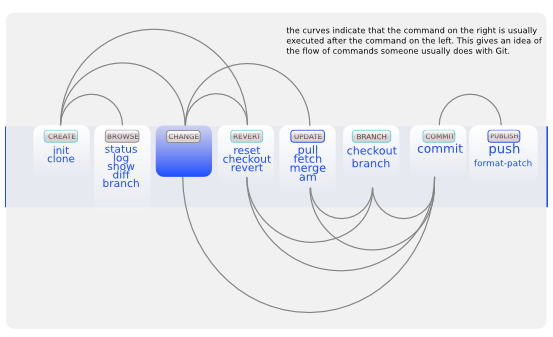
\includegraphics[width=100mm]{./Img/GitCycle.png}
			% GitCycle.png: 0x0 pixel, 0dpi, 0.00x0.00 cm, bb=
			\caption{Cycle de vie Git}
		\end{figure}

		
	\end{frame}
	
	\begin{frame}{Cycle de vie d'un fichier}
		\begin{figure}
			\centering
			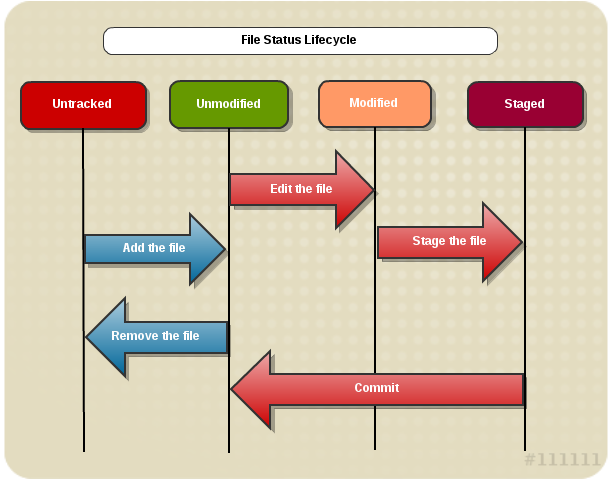
\includegraphics[width=85mm]{./Img/GitLife.png}
			% GitLife.png: 0x0 pixel, 0dpi, 0.00x0.00 cm, bb=
			\caption{Cycle de vie Git d'un fichier}
		\end{figure}

	 
	\end{frame}
\subsection{Commandes}


	\begin{frame}[fragile]{Variables globales}
		\begin{block}<1->{La branche de développement par défaut}
			\verb'master'
		\end{block}
		\begin{block}<2->{Le dépot par défaut}
			\verb'origin'
		\end{block}
		\begin{block}<3->{La branche courante}
			\verb'HEAD'
		\end{block}
	\end{frame}
	

	
	\begin{frame}[fragile]{Notation}
		\begin{block}<1->{Réprésentation de l'id d'un commit, d'une branche ou d'un tag}
			\verb'$id'
		\end{block}
		\begin{block}<2->{Un fichier}
			\verb'$file'
		\end{block}
		\begin{block}<3->{Une branche}
			\verb'$branch'
		\end{block}
	\end{frame}

		\begin{frame}[fragile]
			\frametitle{Create}
			\begin{block}<2->{À partir de données existantes}
				\verb'cd ~/workspace/monprojet'\\
				\verb'git init'\\
				\verb'git add.'
			\end{block}
			\begin{block}<3->{À partir d'un dépot existant}
				\begin{exampleblock}{Le dépot est sur la machine locale}<4>
					\verb'git clone ~/existing/repo ~/new/repo'\\
				\end{exampleblock}

				\begin{exampleblock}{Le dépot est sur une machine distante}<5>
					\verb'git clone git://host.org/project.git'\\
					\verb'git clone ssh://you@host.org/proj.git'
				\end{exampleblock}
			\end{block}

		\end{frame}
		

	
		\begin{frame}[fragile]
			\frametitle{Browse}
			
			\begin{block}<2->{Connaitre les fichiers modifiés dans le dossier}
				\verb'git status'
			\end{block}
			
			\begin{block}<3->{Connaitre les modifications sur les fichiers suivis}
				\verb'git diff'
			\end{block}
			\begin{block}<4->{Connaitre l'historique des modifications}
				\verb'git log'
			\end{block}
			\begin{block}<5->{Connaitre le détail d'un commit}
				\verb'git show $id'
			\end{block}
			\begin{block}<6->{Connaitre toutes les branches locales}
				\verb'git branch'
			\end{block}
		\end{frame}

		\begin{frame}[fragile]
			\frametitle{Revert}
			\begin{block}<2->{Repartir au dernier commit}
				\verb'git revert HEAD'
			\end{block}
			\begin{block}<3->{Repartir à un commit donné}
				\verb'git revert $id'
			\end{block}
			\begin{alertblock}<4->{Retourner à un commit donné}
				\verb'git reset --hard'\\
				\only<5->{Un 'revert' peut être annulé. Un 'reset' NON!}
			\end{alertblock}
			



		\end{frame}

		\begin{frame}[fragile]
			\frametitle{Update}
			\begin{block}<2->{Connaitre les dernières modifications par rapport à origin}
				\verb'git fetch'
			\end{block}
			\begin{block}<3->{Récupérer les dernières modifications par rapport à origin}
				\verb'git pull'
			\end{block}
		\end{frame}

		\begin{frame}[fragile]
			\frametitle{Branch}
			\begin{block}<2->{Passer à une branche donnée}
				\verb'git checkout $id'
			\end{block}
			\begin{block}<3->{Créer une nouvelle branche à partir de l'actuelle}
				\verb'git branch $branch'
			\end{block}
			\begin{block}<4->{Créer une nouvelle branche à partir d'une branche donnée(\$other) et passer sur la nouvelle}
				\verb'git checkout -b $new_branch $other'
			\end{block}
			\begin{alertblock}<5->{Supprimer une branche}
				\verb'git branch -d $branch'
			\end{alertblock}

			
		\end{frame}

		\begin{frame}[fragile]
			\frametitle{Commit}
			\begin{block}<2->{Valider des changements}
				\verb'git commit -m "message"'\\
				L'option \verb'-m' permet d'ajouter un message au commit				
			\end{block}
			\begin{alertblock}<3->{IMPORTANT}
				Les changements que l'on valide sont ceux que l'on a ajouté grâce à \verb'git add $file'\\
				On peut ajouter dans un commit tous les fichiers suivis avec l'option \verb'-a'
			\end{alertblock}
			
		\end{frame}

		\begin{frame}[fragile]
			\frametitle{Publish}
			\begin{block}<2->{Envoyer les changements sur le serveur}
				\verb'git push origin $branch'\\	
			\end{block}
		\end{frame}
		
		\begin{frame}[fragile]
		  \frametitle{Pour le reste}
		  
		  \begin{block}{}
		   \verb'man git'
		  \end{block}
		  
		\end{frame}


